\section{Module}\label{subs:module}
As a configuration is made up of individual modules, it seems natural to model it as a set of synchronizing module processes. In this section we will first show off the initial design of the \textit{Module} template. Then discuss, how we got more concrete with the final version. 

\subsection{Early Module Template}
In our early design work, we tried to implement most everything brought up in \cref{sec:runningexample}. A module has an identifying name, and it may only work on one item at a time. It also takes a certain amount of time to perform  work and to transport an item across it. However, we start by allowing modules to only perform one type of work. There are also no physical restrictions, on which modules may be connected, other than the fact that a module may not be connected to more than four other modules. These basic ideas turned into our first version of the \textit{Module} template, which can be seen in \cref{fig:earlymodule}.


\begin{figure}[h]
\centering
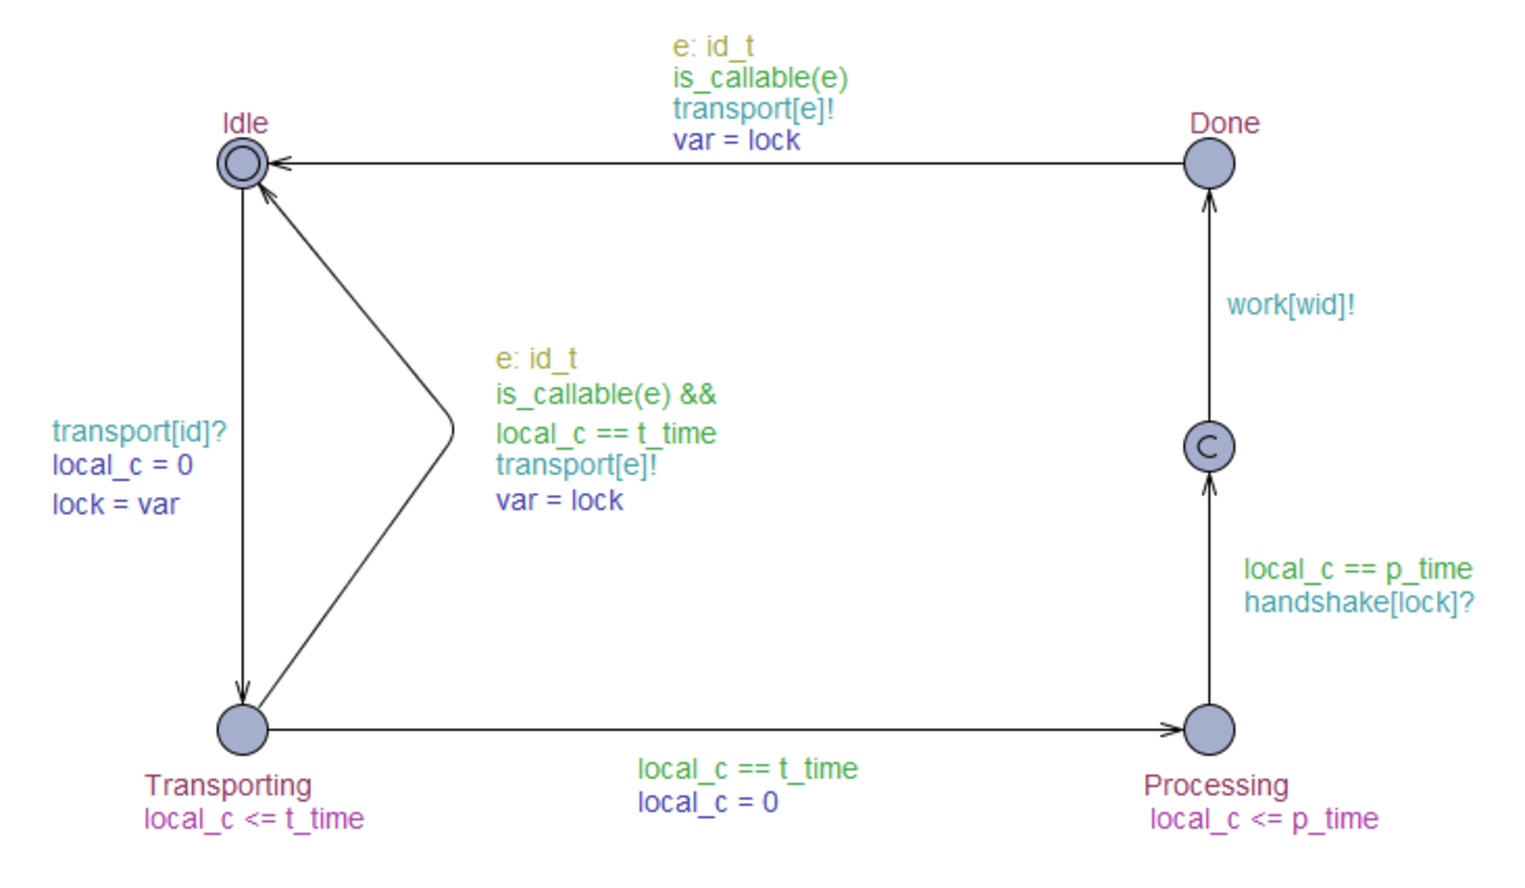
\includegraphics[width=\textwidth]{earlymodule.pdf}
\caption{Early version of the \textit{Module} template}
\label{fig:earlymodule}
\end{figure}

A module starts in the \emph{Idle} location and resides there, when not processing an item. It leaves this location, when one of its up to four neighbouring modules passes on an item by synchronizing on the \emph{transport} channel identified by the modules's id. Once an item has been received, the module waits in the \emph{transporting} location for \emph{t\_time}. This simulates the time taken to transport the item across the module. Once the time has passed we may send the item to a neighbouring module. The local guarding function \emph{is\_callable} makes sure, we only send to neighbours. This set-up allows us to implement modules, which are only used for transporting item.

Instead of passing an item along, we may perform work on it by moving into the \emph{Processing} location. Here we wait for \emph{p\_time}, to simulate the time it takes to work the item. Before we can update the item to have its work performed, it must identify itself. This is done by synchronizing on the \emph{handshake} channel given by the value stored in the local \emph{lock} variable. This variable contains the unique id of the item, which most recently entered the module. It was received from the previous module over the global \emph{var} variable. This ensures that after a handshake, moving us to a committed location, the synchronizing on the \emph{work} channel will be with the correct item. Once work has been performed, we may pass the item onto another module. 

Some modules may also allow for items to be removed from the system by transporting on the reserved \emph{transport[0]} channel. No actual module has the id 0. Instead a process instantiated from the \emph{Remover} template is constantly calling on the \emph{transport[0]} channel. If a synchronization is established the item is removed from the module and not passed on to any other module. A module can only synchronize with the remover process, if it has one of its neighbouring modules set to 0. 

\subsection{Final Module Template}
From further observations of the local CP Learning Factory configuration, we conclude that the above implementation is too abstract. In an actual factory, each module may perform several different types of work on an item, as stated earlier. While only one item is worked at a time, several items may queue up on the module, waiting to be worked on or pass through. A module has a fixed limit of items, which may queue up. This is in accordance with the safety property of the system. If this is not upheld, items may fly off the modules, or the modules themselves may be damaged. Some modules do not allow for items to pass through them, while they are working on another item. This feature is not enforced in the above implementation. In addition, the time to transport an item across a module depend on the dimensions of the module as well as the directions, from which a item enters and leaves.

These features lead to some drastic changes in the module template. The biggest is that the template now gets split into three. \emph{ModuleQueue}, which controls the enqueuing and dequeuing of items. Then \emph{ModuleWorker} which performs work upon a item. Finally \emph{ModuleTransporter}, which transports items between modules. To get a complete module, we need a process of each of these templates sharing the same module id. In the following we will explain each of these new templates.

One aspect that we ultimately do not try to model in UPPAAL are the more extensive physical rules for placing down modules. We choose to enforce these later, when generating and comparing configurations. 

\subsubsection{ModuleQueue Template}\label{subs:modulequeue}
One of the most important characteristics observed was the queuing nature of the system. Several items may be located on a module, but only one is being processed at a time. Some of the items queued may need to be processed, others just want to be passed along to a neighbouring module. Based on this behaviour, we construct the \emph{ModuleQueue} template, which can be seen on \cref{fig:modulequeue}. A process of this template has a fixed size of modules, which it may hold. Other modules may be able to use the \emph{enqueue} channel to move an item onto the module. In addition, items may be removed from it through a synchronization on its \emph{dequeue} channel.

As in the earlier version, an item is moved between instances by proxy of its id. The id is always stored in the local \emph{lock} variable.   

\begin{figure}[h]
\centering
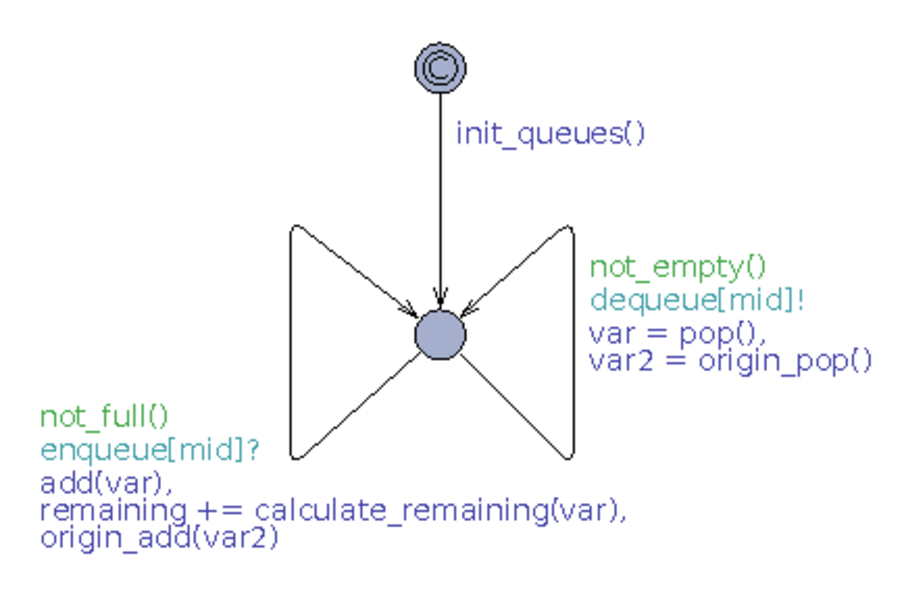
\includegraphics[width=\textwidth]{modulequeue.pdf}
\caption{The \textit{ModuleQueue} template}
\label{fig:modulequeue}
\end{figure}


\subsubsection{ModuleWorker Template}\label{subs:moduleworker}
The \emph{ModuleWorker} template can be seen in \cref{fig:moduleworker}. An instance of this template may apply several different types of work upon an item. In the \textit{Idle} location, the worker waits to synchronize with the module's \emph{ModuleQueue} instance allowing it to enter the \textit{Done} location. If the module can perform some work, it will move into the \emph{Working} location. Here it will wait for \emph{p\_time}, symbolising the time it takes to perform the work. When the wait is over, it will try to synchronize with the item through the \emph{handshake} and \emph{work} channels as in the earlier version. Arriving at the \emph{Done} location, we may choose to work the item further if possible. Otherwise we perform a synchronization on the module's \emph{intern} channel. This passes the item over to the module's \emph{ModuleTransporter} instance. Synchronization on the intern channel may also occur, if the module can not perform any work on the item. This models the case, where an item has to pass through a module without having worked performed, while the model does not allow for pass through while it is working on other items.

\begin{figure}[h]
\centering
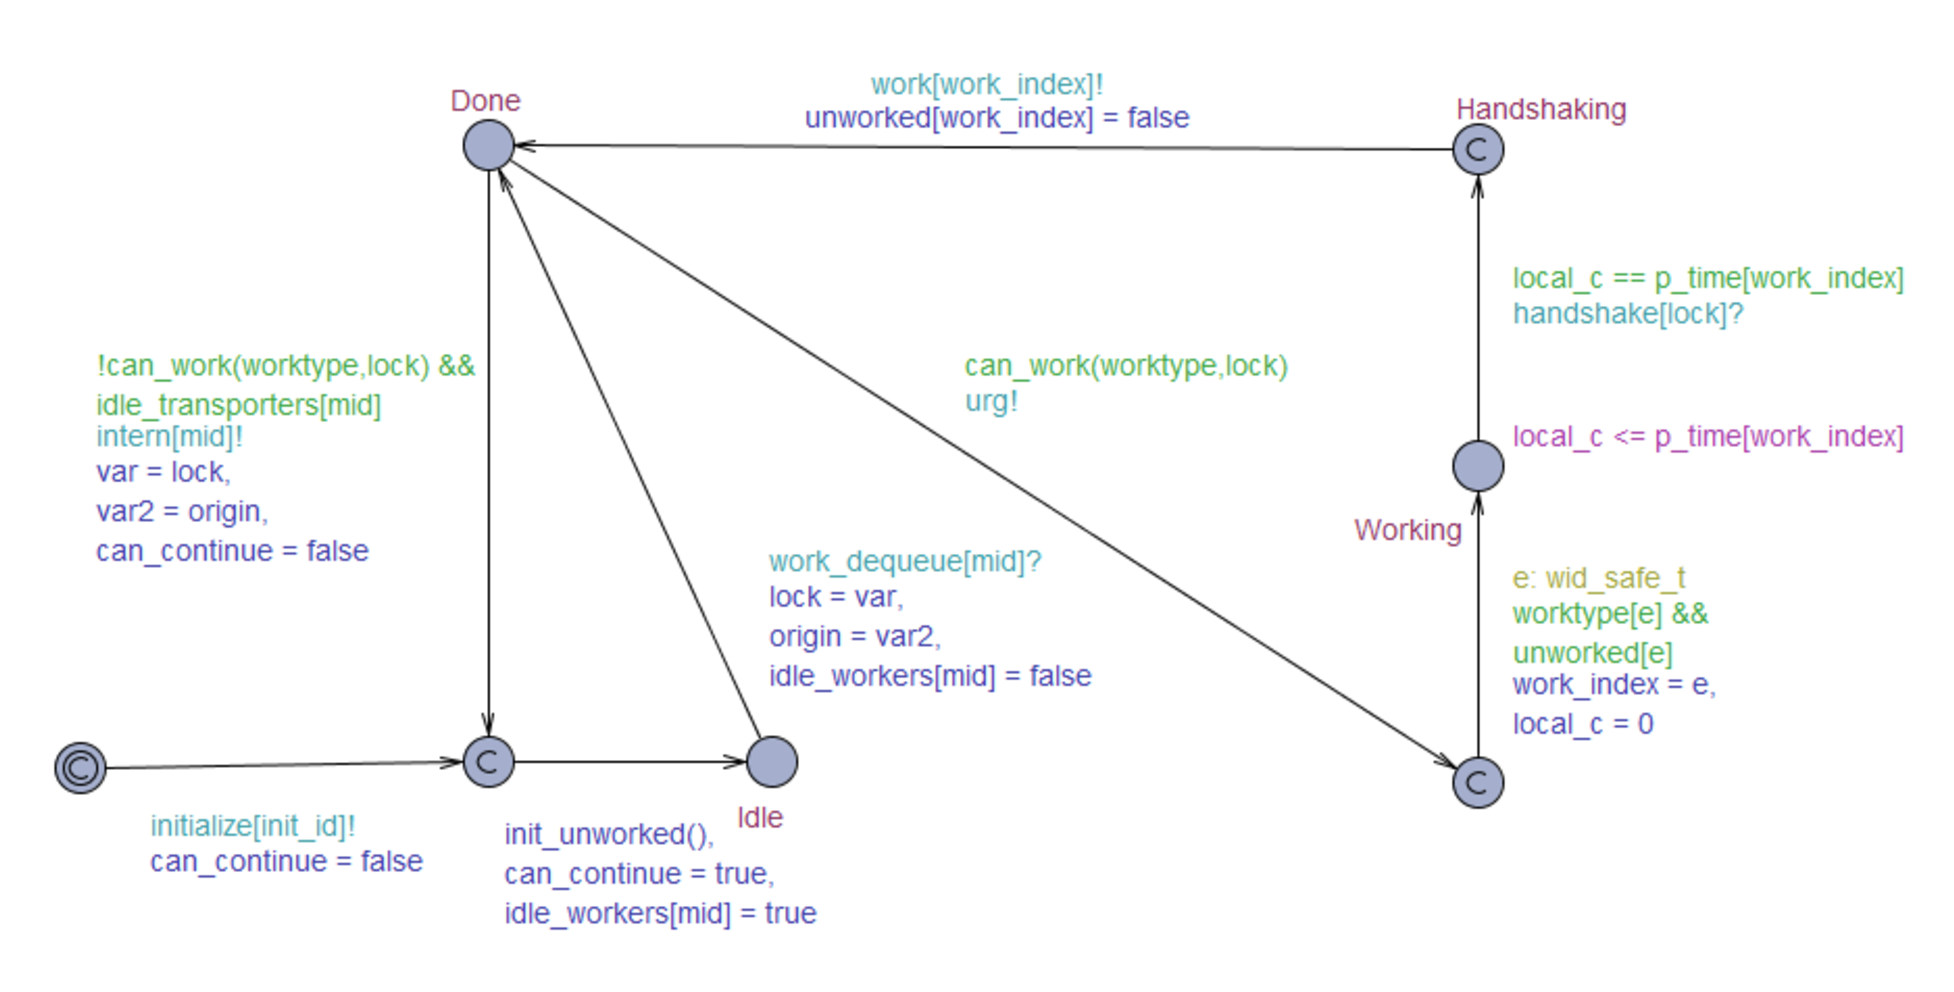
\includegraphics[width=\textwidth]{moduleworker.pdf}
\caption{The \textit{ModuleWorker} template}
\label{fig:moduleworker}
\end{figure}

\subsubsection{ModuleTransporter Template}
The \emph{ModuleTransporter} template can be seen in \cref{fig:moduletransporter}. A process of this template allows a module to transport an item onto a neighbouring module. If the item comes from the module's \emph{ModuleWorker} instance, then we move into the \emph{Selector} location by synchronizing on the module's \emph{intern} channel. We may however also move directly to the \emph{Selector} location by synchronizing with the module's \emph{ModuleQueue} instance over the \emph{dequeue} channel. This can however only be done, if the \cref{fig:moduletransporter} module allows us to pass an item through a module, while it is working on another item. This is indicated by the boolean \emph{pass\_through} variable, which is given at process instantiation. To create a module only used for transportation, we set this variable to \emph{true} and do not create a \emph{ModuleWorker} instance for the module. 

Once in the \emph{Selector} location a item may go to \emph{Idle} or \emph{Transporting}. If the item is done, it has to go back to \textit{Idle} and be removed from the production line by synchronizing on the \emph{remove} channel, as opposed to the \emph{transport[0]} in the earlier version. This also means that we do not specify a specefic module to remove items from, they are just removed when done.

If the item is not done, it may look for a neighbouring module to be passed onto. A module may have up to four neighbours, one on each side. These are stored in the local \emph{next} array, their index indicating their placement relative to the module. When moving to \emph{Transporting} location, the item will choose a possible neighbour. In \emph{Transporting}, we wait to simulate the time taken to transport an item over the module. This time varies according to where the item enters the module, and where it leaves. The different transport times are stored in the 4 by 4 multidimensional \emph{t\_time} array. Given that we at this point know the direction, which the item entered from \emph{origin}, and the direction on which it will leave \emph{succ}, we can look up the exact time to wait in \emph{t\_time}. By implementing this feature, we ensure that the time take to pass over a module becomes more accurate to how an item may actually be transported over a module. 

Once the wait is over we move to the \emph{Queuing} location. If the neighbour's queue is full, we wait here until there is room. When possible we synchronize with the neighbours instance of \emph{ModuleQueue} using the \emph{enqueue} channel. At the same time we use the local \emph{inverse} function to calculate, from which side the item enters the neighbouring module. This is sent with the global \emph{var2} variable and is later saved into the  \emph{origin} variable of the neighbour's \textit{ModuleQueue} process. 

\begin{figure}[h]
\centering
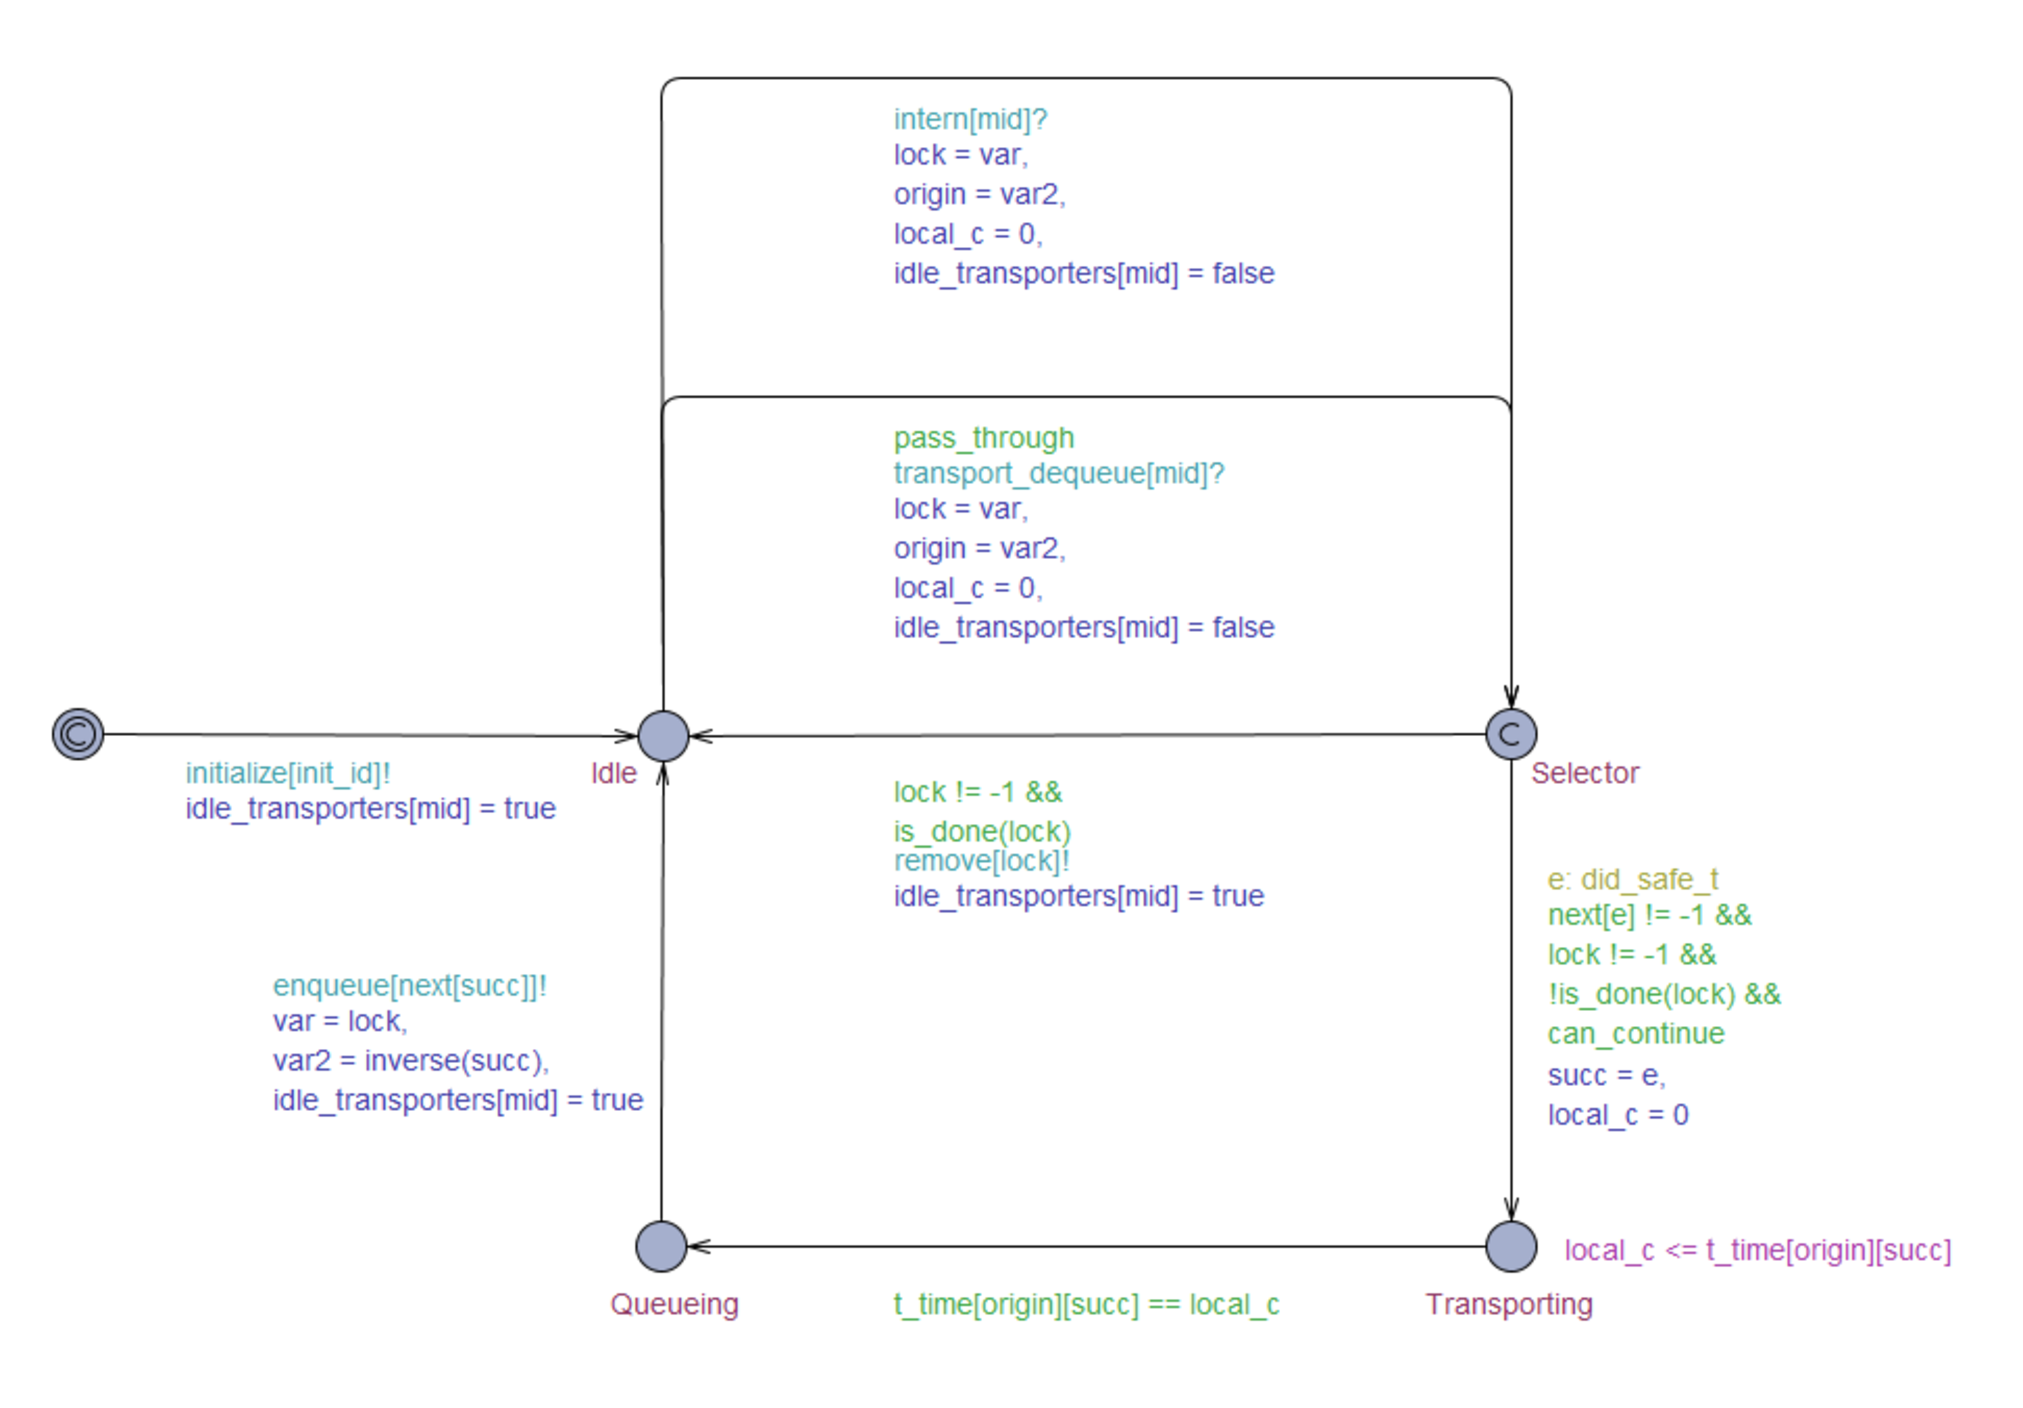
\includegraphics[width=\textwidth]{moduletransporter.pdf}
\caption{The \textit{ModuleTransporter} template}
\label{fig:moduletransporter}
\end{figure}


